\documentclass[12pt,english]{article}
\usepackage{geometry}
\usepackage{float}
\usepackage{caption}
\geometry{verbose,tmargin=3cm,bmargin=3cm,lmargin=3cm,rmargin=3cm}
\usepackage{amsmath}
\usepackage{amssymb}
\usepackage{amsthm}
\usepackage{adjustbox}
\usepackage{hyperref}
\usepackage{graphicx}
\usepackage{setspace}
\usepackage{changepage}
\onehalfspacing
\usepackage{babel}
\newcommand{\expec}{\ensuremath{\mathbb E}}
\begin{document}
\begin{center}
{\Large{}Section 2: Evidence for slack} \\
{\large{}Schilbach (2015) and Schofield (2014)}
\par\end{center}{\Large \par}

\begin{center}
EEP 152
\par\end{center}

\begin{center}
September 7, 2016
\par\end{center}

\begin{itemize}
	\setlength\itemsep{-0.5em}
	\item Introduction (10 min)
	\item Schilbach (2015) and discussion (20 min)
	\item Schofield (2014) and discussion (20 min)
\end{itemize}
Copies of the two papers, downloaded from the authors' websites, are available on the section Github at \href{github.com/johnloeser/eep152}{github.com/johnloeser/eep152} in the ``section2'' folder. If you missed the first section, it would be useful to briefly go through the section syllabus, also available on the section Github.

\section{Introduction}

In the past section, we talked about potential explanations for the large gap in incomes between rich and poor countries, focusing on macroeconomic poverty traps. In class on Wednesday, we moved to the microeconomic level, instead focusing on how to explain the existence of what are often called ``poverty'' (consumption $<\$2$/day) and ``extreme poverty'' (consumption $<\$1$/day). Does the Solow logic still apply -- should we expect the poor and extreme poor to be able to save a little, invest a little, and earn huge returns on those investments?

We noted two necessary conditions for this to hold. First, the poor must be able to save. Alternatively phrased, the subsistence constraint (the level of consumption needed to survive) must not bind for the poor. Banerjee and Duflo, in ``The Economic Lives of the Poor'', conduct a budgeting exercise to consider this, and conclude that the poor are potentially able to save, either through reducing less necessary expenditures (such as on entertainment, festivals, alcohol and tobacco) or by adjusting their food expenditures (spending less on expensive sources of calories, such as rice, sugar, and wheat, and spending more on cheaper sources of calories, such as millet). Second, the poor must be able to accumulate capital.

Today, we'll discuss the first condition. Specifically, we'll ask the question ``is there `slack' in the budgets of the poor'' through the lens of two recent papers studying cycle rickshaw drivers in Chennai, India. This is a population of middle-aged men, typically married with children, with low levels of education, and slightly above the \$2/day consumption poverty line. Both use a methodology called a randomized controlled trial (RCT), which we'll discuss more in class next week. In short, in an RCT, groups or individuals (in our case, individual cycle rickshaw drivers) are randomly assigned to one of two groups -- treatment (where some treatment is applied), or control (where nothing is done). To calculate the effects of the treatment (in the case of these two papers, incentives to abstain from alcohol and extra calories, respectively) on a particular outcome (in the case of these two papers, savings and income, respectively), the difference in average outcomes between the treatment group and the control group is calculated. We can then conclude that this difference is the effect of the treatment, since assignment to either the treatment group or the control group was random.

\begin{figure}[H]
\begin{center}
\begin{adjustbox}{
		max width=0.65\textwidth,
	}
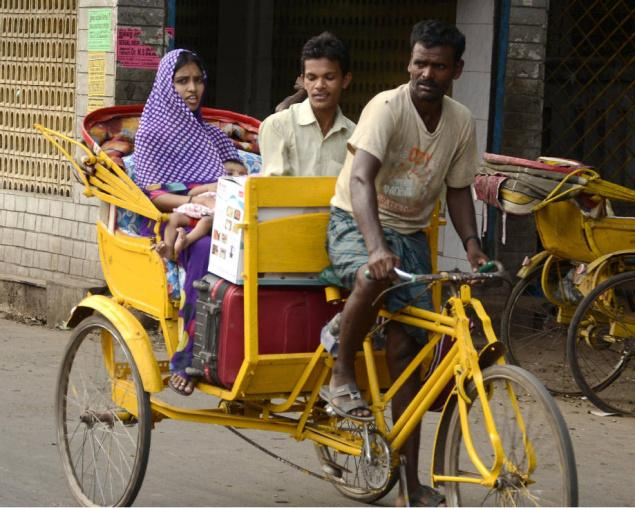
\includegraphics{cyclerickshaw.jpg}
\end{adjustbox}
\end{center}
\begin{adjustwidth}{0.175\textwidth}{0.175\textwidth}
\href{http://www.thehindu.com/news/cities/chennai/at-the-cycle-rickshaw-stand-it-is-business-as-usual/article3466786.ece}{http://www.thehindu.com/news/cities/chennai/at-the-cycle-rickshaw-stand-it-is-business-as-usual/article3466786.ece}
\end{adjustwidth}
\end{figure}

The first, ``Alcohol and Self-Control'' (Schilbach (2015)), asks whether consumption of alcohol directly causes self-control problems, reducing individuals' ability to save. The second, ``The Economic Costs of Low Calorie Intake'', asks whether increasing caloric consumption can increase productivity. (How do each of these fit into our necessary conditions for applying Solow style reasoning to the microeconomics of the poor?)

\section{Schilbach (2015) -- Alcohol and Self-Control}

As mentioned in ``The Economic Lives of the Poor'', there is some evidence that the poor have self-control problems. While this is true of people in general, the stakes may be higher for the poor if they have an extremely high marginal return to capital, as Solow style reasoning would suggest. The poor report spending money on less necessary expenditures that they would rather have saved. Alcohol is known to contribute to self-control problems, and additionally is one of those less necessary expenditures that the poor have been documented to make. Can this potentially generate a poverty trap, where the poor spend money on alcohol, which in turn reduces their self-control, which in turn makes it more difficult to save instead of spending more money on alcohol?

Schilbach studies a population of cycle rickshaw drivers who consistently consume alcohol, reporting average consumption of between 3 and 9 standard drinks per day (and spending about \$1.50/day on average on alcohol). The drivers were asked to come into a lab-in-the-field in Chennai, complete a survey, and be breathalyzed daily. All drivers were also offered a high interest savings account at the lab. Additionally, two randomizations occured. First, drivers were placed into one of three groups -- control, incentives (paid \$1/day if they blew a 0 on the breathalyzer), and choice (paid \$1/day if they blew a 0 on the breathalyzer during week 1, then offered choice between being paid \$1/day if they blew a 0 on the breathalyzer and a guaranteed payment of either \$0.50, \$1, or \$1.50). Second, drivers were additionally placed into one of two groups -- control, or commitment savings (money placed in the high interest savings account could only be withdrawn at the end of the study period).

\begin{figure}[H]
	\begin{center}
		\begin{adjustbox}{
				max width=\textwidth,
			}
			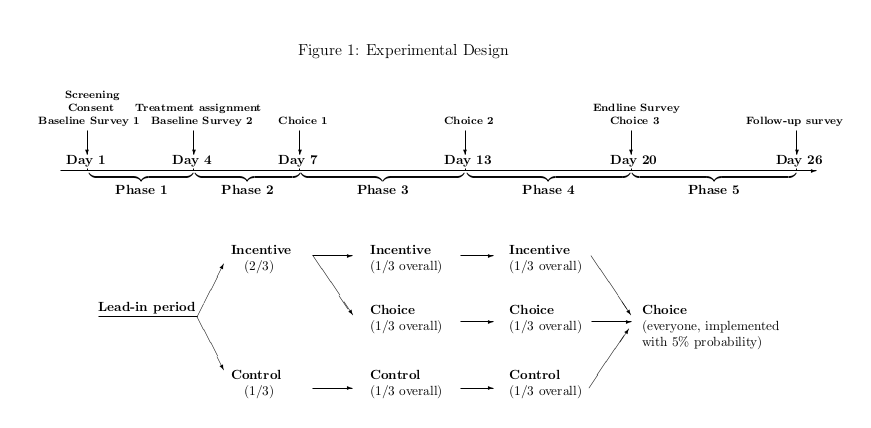
\includegraphics{schilbachfig1.png}
		\end{adjustbox} \\
		Schilbach (2015), Figure 1
	\end{center}
\end{figure}

A few key findings. First, commitment savings and incentives to abstain from alcohol both increase savings in the experiment. However, they appear to be substitutes - individuals receiving both incentives to abstain and the commitment savings account did not save any more than individuals receiving either one or the other.

\begin{figure}[H]
	\begin{center}
		\begin{adjustbox}{
				max width=0.8\textwidth,
			}
			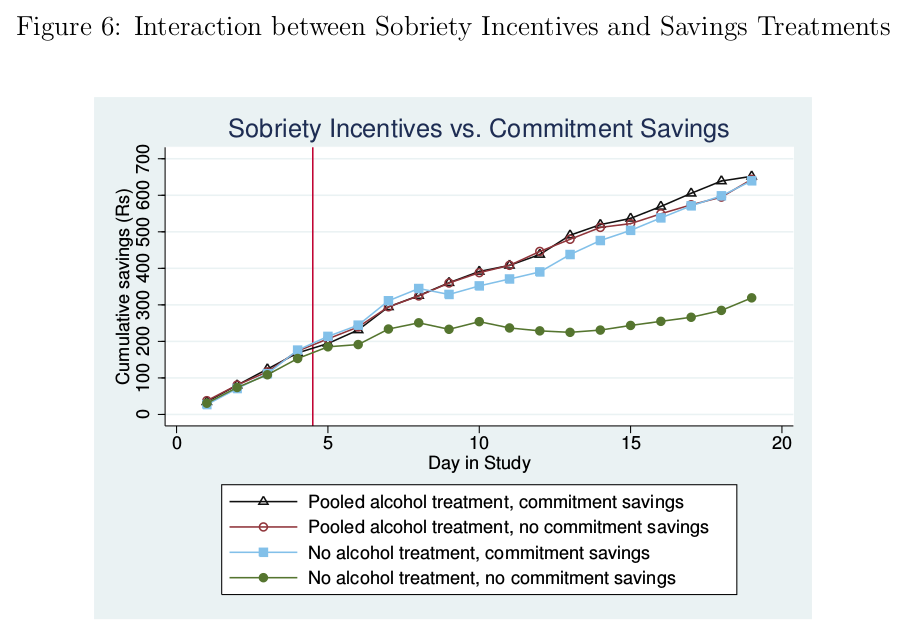
\includegraphics{schilbachfig6.png}
		\end{adjustbox} \\
		Schilbach (2015), Figure 6
	\end{center}
\end{figure}

Second, about 40\% of individuals in the experiment would prefer having a \$1 incentive to abstain from alcohol to a \$1.50 guaranteed payment, and the demand for this incentive was increasing with sobriety.\footnote{This is measured either using observed variation in sobriety, which is not random, or using variation in sobriety randomly induced by the strength of the incentives.}

How do these results tie into ``The Economic Lives of the Poor''? How should we think about these results? What should we learn from them?

\section{Schofield (2014) -- The Economic Costs of Low Calorie Intake}

``The Economic Lives of the Poor'' discusses a few ideas about the food consumption of the poor. First, it mentions that there appears to be budgetary slack in the food choices of the poor -- many of the poor consume more expensive sources of calories (rice, sugar, wheat) instead of cheaper sources of calories (millet). Second, it speculates that increasing consumption of food may increase productivity, especially somewhere like India (where many of the poor are underweight), so it seems surprising that many of the poor appear to save to make entertainment purchases rather than spending now on increasing low levels of food consumption.\footnote{While this may seem to contradict the self-control problems documented in Schilbach (2015), there is no monolithic model of the behavior of the poor -- one model may be reasonable in some contexts for some individuals, while another model may hold elsewhere for others.}

Schofield studies a similar population of cycle rickshaw drivers with low BMI. Similar to Schilbach (2015), the drivers were asked to come into a lab-in-the-field in Chennai and complete a survey daily. Additionally, drivers were randomly placed into one of two groups -- control, and calories (given 700 calories of food each day, asked to consume food in the lab).

The key finding is that the increased calories led to increases in hours worked and earnings, although these effects needed a few weeks to take hold. Importantly, the increased earnings per day measured in the 5th week (about \$0.25) is approximately double the cost of the calories provided in the experiment, suggesting high returns to additional expenditures on calories.

\begin{figure}[H]
	\begin{center}
		\begin{adjustbox}{
				max width=\textwidth,
			}
			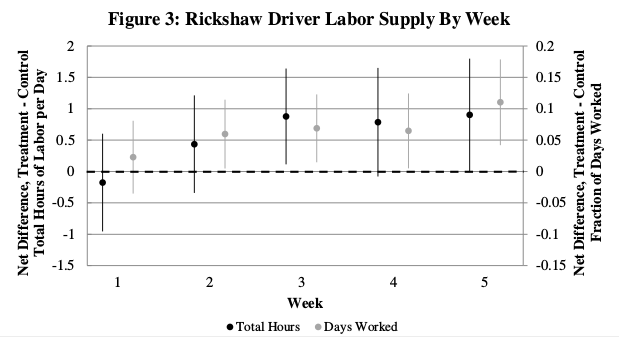
\includegraphics{schofieldfig3.png}
		\end{adjustbox}
		\begin{adjustbox}{
				max width=\textwidth,
			}
			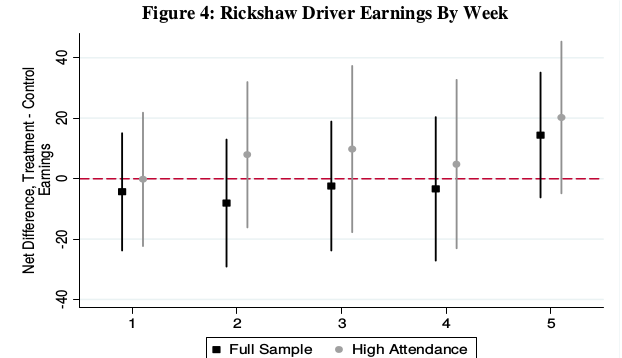
\includegraphics{schofieldfig4.png}
		\end{adjustbox} \\
		Schofield (2014), Figures 3 and 4
	\end{center}
\end{figure}

How do these results tie into ``The Economic Lives of the Poor''? How should we think about these results? What should we learn from them?

\end{document}